We would like to start our thesis with a general description of the
communication structure between an actors among with possible security and user privacy vulnerabilities.
Communication model of the instant messaging system is a quite large topic since it implies various protocols, approaches etc,
therefore current discussion asserts the communication over HTTP protocol via REST API\@ using JSON data format.
Since that main task of this thesis is to implement software components that meet the specified security requirements,
namely: \textit{Web Client, Web API, Mobile client, Desktop client} which are
considered to be the actors we focus our attention to.
The following diagram describes the basic concept of the system and conveys the relationships between the
actors mentioned above.

\begin{figure}[H]
    \centering
    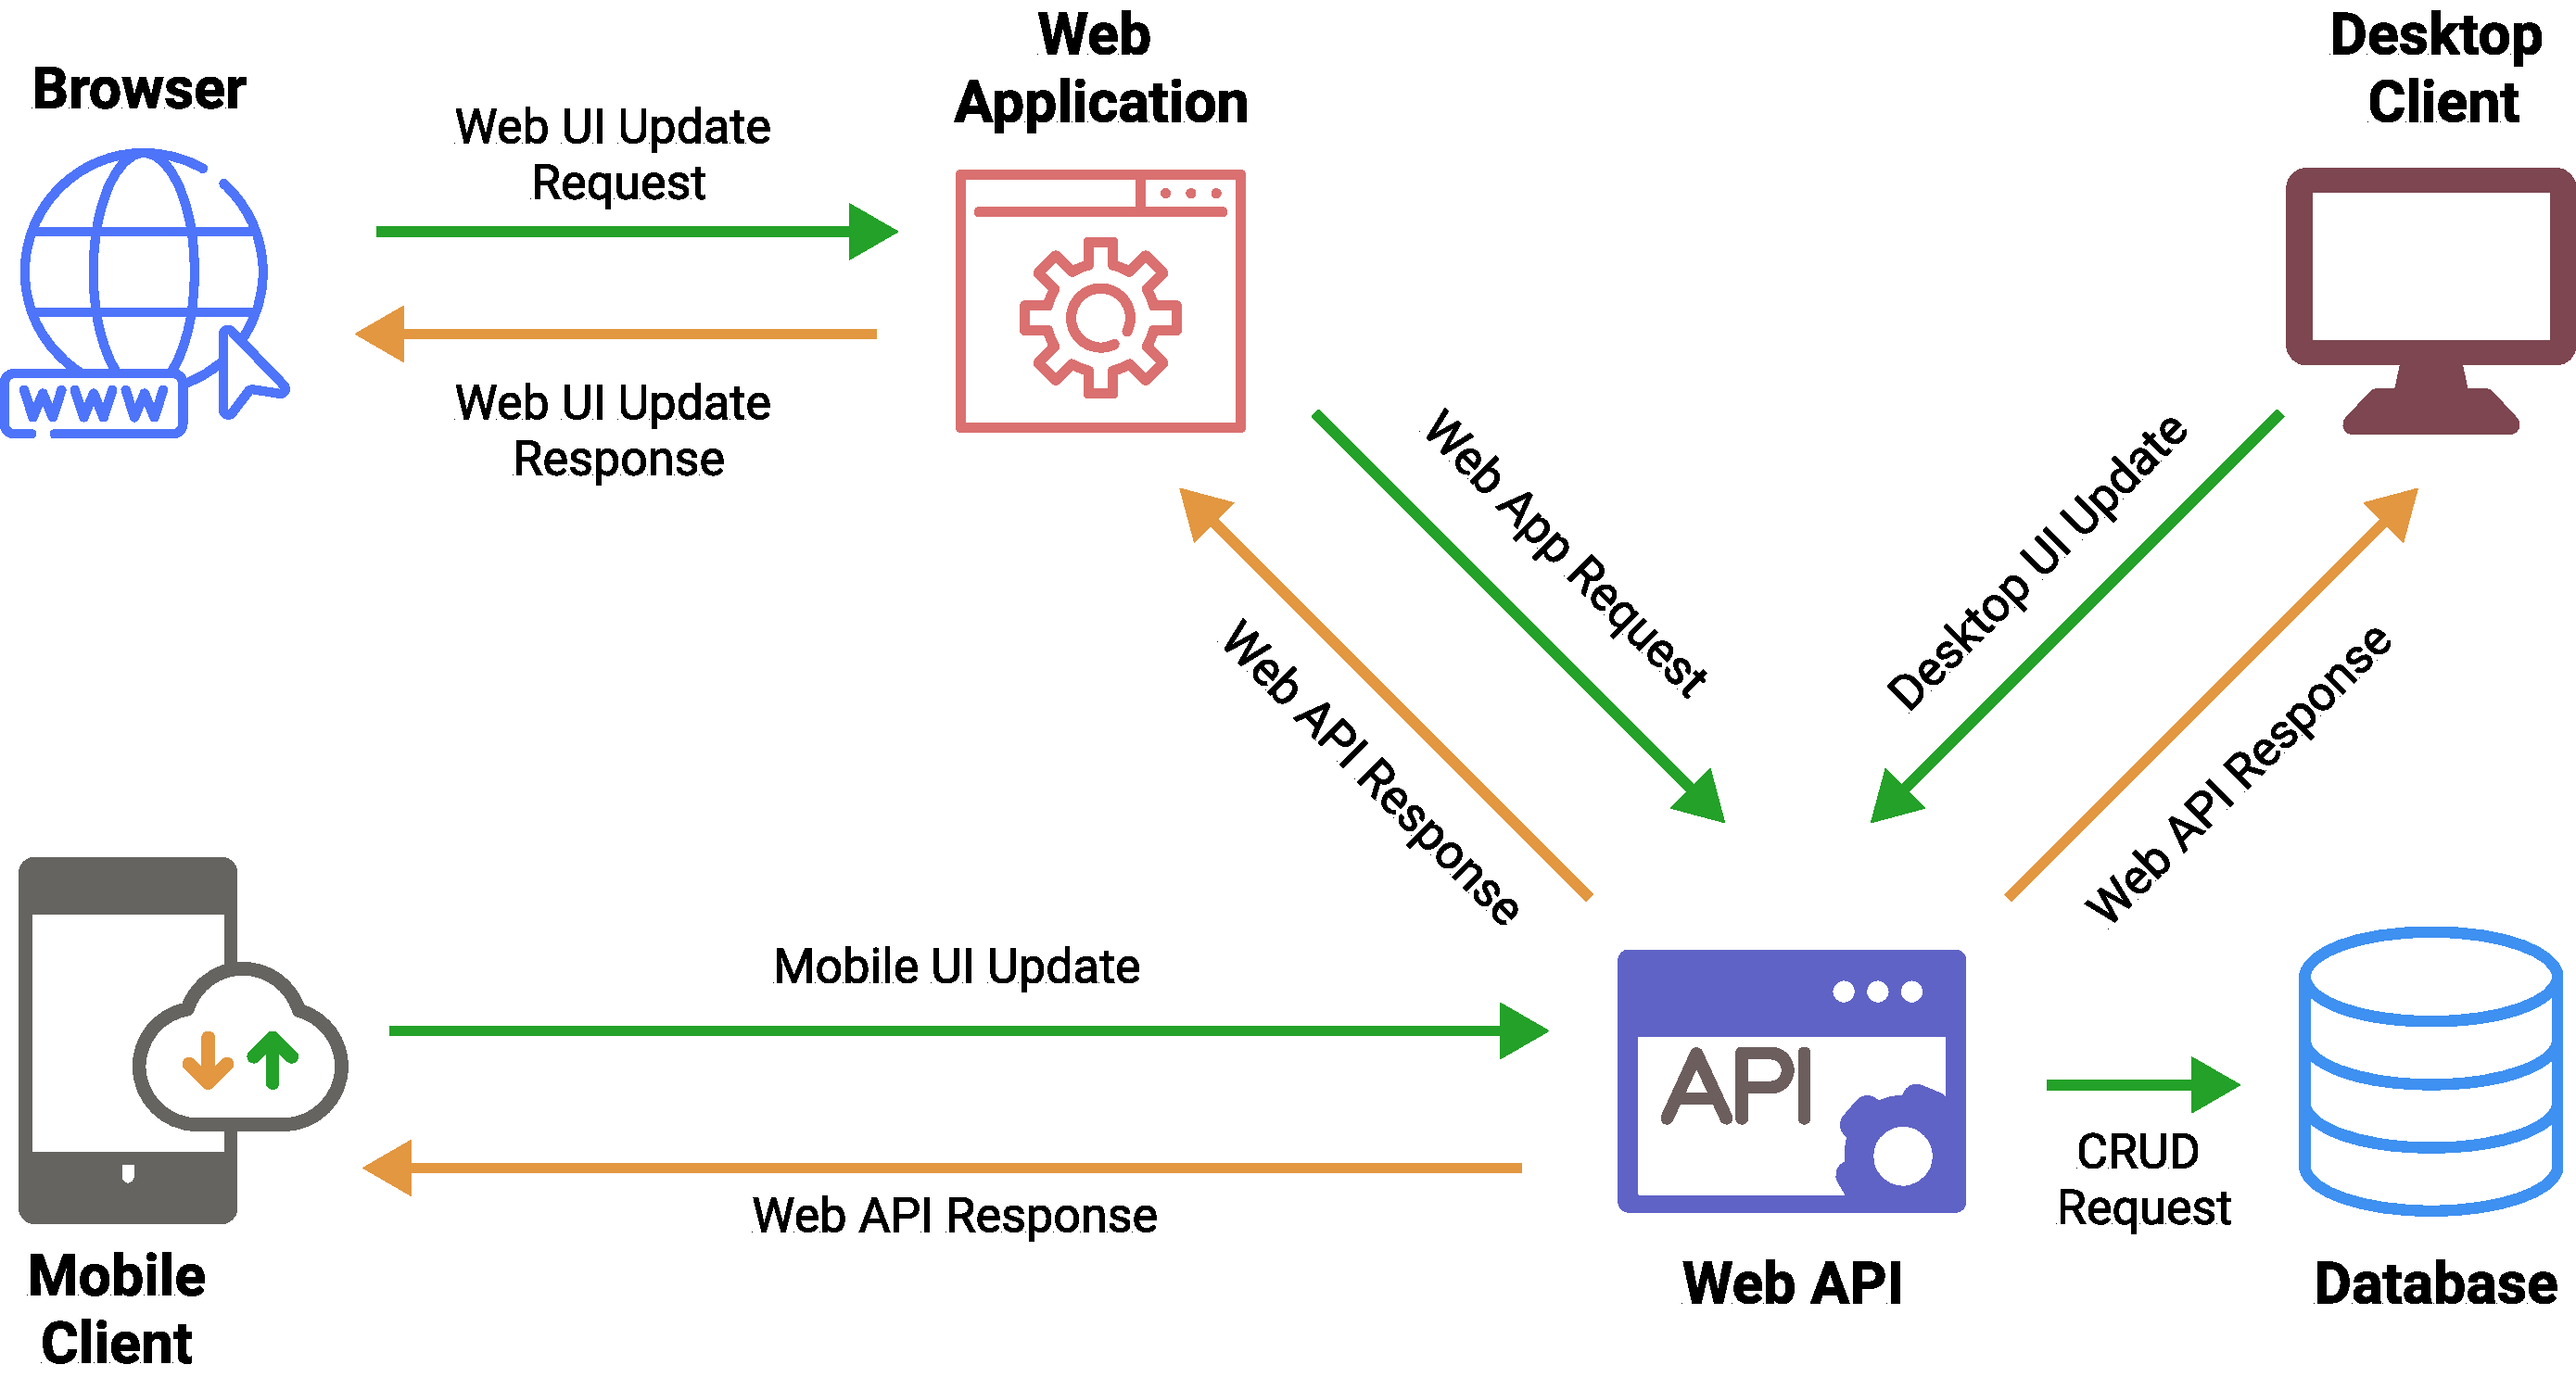
\includegraphics[width=1\textwidth]{Pictures/01_Software_modules_communication_diagram}
    ~\caption{Software modules communication diagram. Source: [\cite{mango2021figma}].}\label{fig:figure6}
\end{figure}

Hence, communication between software components is organised as follows\\

\textit{Browser -- Web Application -- Web API -- Database communication model}
\begin{itemize}
    \item Browser downloads application static files from Web Application server.
    \item Browser sends a request to Web API\@.
    \item Web API checks access rights, executes business logic referring to the Database.
    \item Web API responds to the Browser.
    \item Browser user interface is being updated.
\end{itemize}

\textit{Desktop Client -- Web API -- Database communication model}
\begin{itemize}
    \item Desktop Client sends a request to update the user interface.
    \item Web API checks access rights, executes business logic referring to the Database.
    \item Web API responds to Desktop Client.
    \item Desktop Client's user interface updated as per response from the Web API\@.
\end{itemize}

\textit{Mobile Client -- Web API -- Database communication model}
\begin{itemize}
    \item Mobile Client sends a request to update the user interface.
    \item Web API checks access rights, executes business logic referring to the Database.
    \item Web API responds to the desktop Mobile Client.
    \item Mobile Client's user interface updated as per response from the Web API\@.
\end{itemize}

However, such communication models are under possible security vulnerabilities, most of which are already fixed
\textit{'out of the box'} in modern web frameworks, so we discuss these are requiring additional attention.
The first vulnerability that comes to mind is phishing [\cite{dhamija2006phishing}].
An attacker could launch his own web application consuming our web API, therefore it is possible to log user actions
and get access to personal data or credentials.
Phishing attack could be mitigated using a properly configured Cross-Origin Resource Sharing [\cite{gibbinscross}]
policy that will restrict the queries from the domains that do not meet the policy.
For instance, in our project the CORS configured as follows

\begin{spverbatim}
    public static void Configure(
    IApplicationBuilder app,
    IWebHostEnvironment env)
    {
        ...

        app.UseCors(CorsPolicy);

        ...
    }

    public void ConfigureServices(IServiceCollection services)
    {
        ...

        services.AddCors(options =>
        {
            options.AddPolicy(CorsPolicy, builder =>
            {
                var allowedOrigins = Configuration
                        .GetSection("AllowedOrigins")
                        .Get<string[]>();

                builder.WithOrigins(allowedOrigins)
                       .AllowAnyMethod()
                       .AllowCredentials()
                       .AllowAnyHeader();
            });
        });

        ...
    }

\end{spverbatim}

The next potential vulnerability is improper SSL certificate configuration [\cite{georgiev2012most, el2012most}]
or usage of self-signed certificate [\cite{kappenberger2012true}],
to eliminate the vulnerability of the improper SSL certificate, it is recommended to follow the instructions
and best practices [\cite{rapp2021web}].

In addition, a potential vulnerability lies in the possibility of SQL injection [\cite{halfond2006classification}].
The SQL injection vulnerability is eliminated by using parameters in string literals of the SQL query.
Also, it is necessary to pay attention to the configuration used ORM [\cite{tiwari2015study}].

There is another danger that attacker may receive information about the application infrastructure
through the error messages in the response from the server, thus, it is recommended to use the unified
response format according to RFC 7231-Hypertext Transfer Protocol [\cite{fielding2014rfc}].
Therefore, in case of an error response will not contain any details.

In order to provide proper authorization, it is recommended to use the roles for users in order to restrict
unauthorized access to the resources available only to administrators.

The last, but not the least possible vulnerability -- is a famous worm and virus spreading problem [\cite{mannan2005instant}].
Obviously, it is not a problem to get rid of the worms in local network with just a few devices connected,
however worms are really dangerous for the huge networks, like messenger considered to be.
The fight against the worms generally dependent on the end-user's security best practices education (at least user should
not use the public unprotected wi-fi networks) and firewall settings of the network.
However, the spread of viruses may be mitigated by the certain validation rules upon file upload such as follows
\begin{spverbatim}
    public UploadDocumentCommandValidator()
    {
        var allowedExtensions = new List<string>
        {
            "jpg", "JPG", "txt", "TXT", "pdf",
            "PDF", "gif", "GIF", "png", "PNG"
        };

        RuleFor(x => x.FormFile).NotEmpty();

        RuleFor(x => x.FormFile.Length)
            .LessThanOrEqualTo(10 * 1024 * 1024);

        RuleFor(x => x.FormFile.FileName)
            .Cascade(CascadeMode.Stop)
            .NotEmpty()
            .Must(t =>
            {
                var validExtension = t.Split('.').Last();
                return allowedExtensions
                .Contains(validExtension);
            }).Length(1, 20);
    }
\end{spverbatim}